
\chapter{Tableau de bord}
\label{chap:dashboard}

\section{Objectifs}

Le tableau de bord constitue un espace de synthèse permettant aux utilisateurs de consulter rapidement les informations essentielles liées à la gestion des consommations et des factures.

Son contenu varie selon le rôle de l'utilisateur connecté. Le fournisseur dispose d'indicateurs financiers et de graphiques permettant de suivre l'activité de ses clients, tandis que le client accède à un résumé de sa propre situation.

\section{Indicateurs fournisseur}

Le tableau de bord du fournisseur présente quatre indicateurs principaux :

\begin{itemize}
    \item \textbf{Total des factures impayées :} montant TTC des factures dont l'état est \texttt{IMPAYEE} pour l'année sélectionnée.
    \item \textbf{Total encaissé :} montant TTC des factures dont l'état est \texttt{PAYEE} pour l'année sélectionnée.
    \item \textbf{Nombre de clients :} nombre de clients rattachés au fournisseur.
    \item \textbf{Anomalies en attente :} nombre d'anomalies dont le statut est \texttt{EN\_ATTENTE}.
\end{itemize}

Ces indicateurs sont calculés à partir des données enregistrées dans la base de données. Les résultats sont affichés sous forme de cartes statistiques afin de faciliter leur consultation.

\section{Total des factures impayées}

Le montant total des factures impayées est calculé en additionnant les montants TTC des factures associées aux clients du fournisseur et dont l'état est \texttt{IMPAYEE}.

Le calcul est réalisé par la méthode \texttt{totaux()} de la classe \texttt{DashboardBD}. Cette méthode utilise une requête SQL avec la fonction d'agrégation \texttt{SUM()} et une condition sur l'état de chaque facture.

Le tableau de bord affiche également le nombre de factures impayées correspondant au montant calculé.

\section{Total encaissé}

Le total encaissé représente la somme des montants TTC des factures dont l'état est \texttt{PAYEE}.

Lorsqu'un fournisseur enregistre le paiement d'une facture, son état est mis à jour dans la base de données. Le tableau de bord prend ensuite en compte ce changement dans le calcul du montant encaissé.

Le nombre de factures payées est également affiché afin de compléter cet indicateur financier.

\section{Évolution mensuelle}

Le tableau de bord permet de suivre l'évolution mensuelle des consommations d'eau et d'électricité facturées pendant l'année sélectionnée.

La méthode \texttt{evolutionMensuelle()} de la classe \texttt{DashboardBD} regroupe les factures par mois à l'aide de la clause SQL \texttt{GROUP BY}. Pour chaque mois, elle calcule :

\begin{itemize}
    \item la somme des consommations d'eau ;
    \item la somme des consommations d'électricité ;
    \item le montant TTC total des factures ;
    \item le nombre de factures correspondantes.
\end{itemize}

La méthode complète ensuite les résultats pour obtenir douze entrées, de janvier à décembre. Lorsqu'aucune facture n'est enregistrée pour un mois, les valeurs correspondantes sont initialisées à zéro.

Cette organisation permet de présenter une évolution annuelle continue, même lorsque certains mois ne comportent aucune facture.

\section{Graphiques}

Les consommations mensuelles sont représentées à l'aide de deux graphiques en barres verticales :

\begin{itemize}
    \item un graphique consacré à la consommation d'eau, exprimée en mètres cubes (m\textsuperscript{3}) ;
    \item un graphique consacré à la consommation d'électricité, exprimée en kilowattheures (kWh).
\end{itemize}

Les graphiques sont générés par la fonction PHP \texttt{chart\_barres()}, définie dans \texttt{config/app.php}. Cette fonction construit directement le code SVG du graphique à partir des données mensuelles fournies.

Chaque graphique représente les douze mois de l'année. La hauteur de chaque barre est proportionnelle à la consommation du mois par rapport à la valeur maximale de l'année. Les noms abrégés des mois sont affichés sous les barres.

Une infobulle SVG permet également d'afficher le nom du mois, la valeur de consommation et son unité lorsque l'utilisateur survole une barre non nulle.

Cette solution utilise le format SVG pour produire les graphiques sans dépendre d'une bibliothèque JavaScript externe.

\section{Filtre par année}

Le fournisseur peut sélectionner une année à partir d'une liste déroulante affichée en haut du tableau de bord.

Les années disponibles sont récupérées par la méthode \texttt{anneesDisponibles()}, qui recherche les années distinctes présentes dans les factures associées aux clients du fournisseur.

Après sélection, le formulaire transmet l'année choisie par une requête HTTP GET. Le contrôleur vérifie que cette année appartient à la liste des années disponibles. Si la valeur demandée n'est pas valide, l'application sélectionne automatiquement l'année la plus récente disponible. En l'absence de factures, l'année courante est utilisée.

Le filtre annuel actualise les montants des factures et les graphiques correspondant à l'année choisie. Le montant total des factures impayées, toutes années confondues, reste également affiché comme information complémentaire.

\section{Tableau de bord client}

Le client dispose d'un tableau de bord simplifié qui présente les informations relatives à son compte.

Trois indicateurs sont affichés :

\begin{itemize}
    \item \textbf{Dernière consommation :} période et statut du dernier relevé enregistré pour le client.
    \item \textbf{Mes factures :} nombre total de factures associées à son compte.
    \item \textbf{Période de saisie :} indique si la période de saisie est ouverte ou fermée.
\end{itemize}

La période de saisie est considérée comme ouverte à partir du 18 du mois. Le tableau de bord affiche également le nombre de jours restants jusqu'à la fin du mois lorsque cette période est ouverte.

Deux raccourcis permettent au client d'accéder directement à la saisie de ses consommations et à la consultation de ses factures.

Concernant les autres rôles, le visiteur non connecté accède à la page d'accueil publique. L'agent est automatiquement redirigé vers son espace d'import annuel.

\section{Tests}

Les scénarios suivants permettent de vérifier le fonctionnement du tableau de bord :

\begin{itemize}
    \item vérifier l'affichage des quatre indicateurs du fournisseur ;
    \item vérifier le calcul des montants impayés et encaissés à partir des états des factures ;
    \item vérifier le nombre de clients et d'anomalies en attente ;
    \item vérifier l'affichage des douze mois dans les graphiques ;
    \item vérifier qu'un mois sans facture présente une valeur nulle ;
    \item vérifier que les graphiques représentent correctement les consommations d'eau et d'électricité ;
    \item sélectionner une autre année et vérifier l'actualisation des indicateurs et des graphiques ;
    \item vérifier le comportement lorsque aucune facture n'est disponible ;
    \item vérifier l'affichage des indicateurs du tableau de bord client ;
    \item vérifier la redirection de l'agent vers son espace d'import annuel.
\end{itemize}

Ces scénarios constituent les vérifications fonctionnelles à effectuer sur le tableau de bord.

\begin{figure}[H]
  \centering
  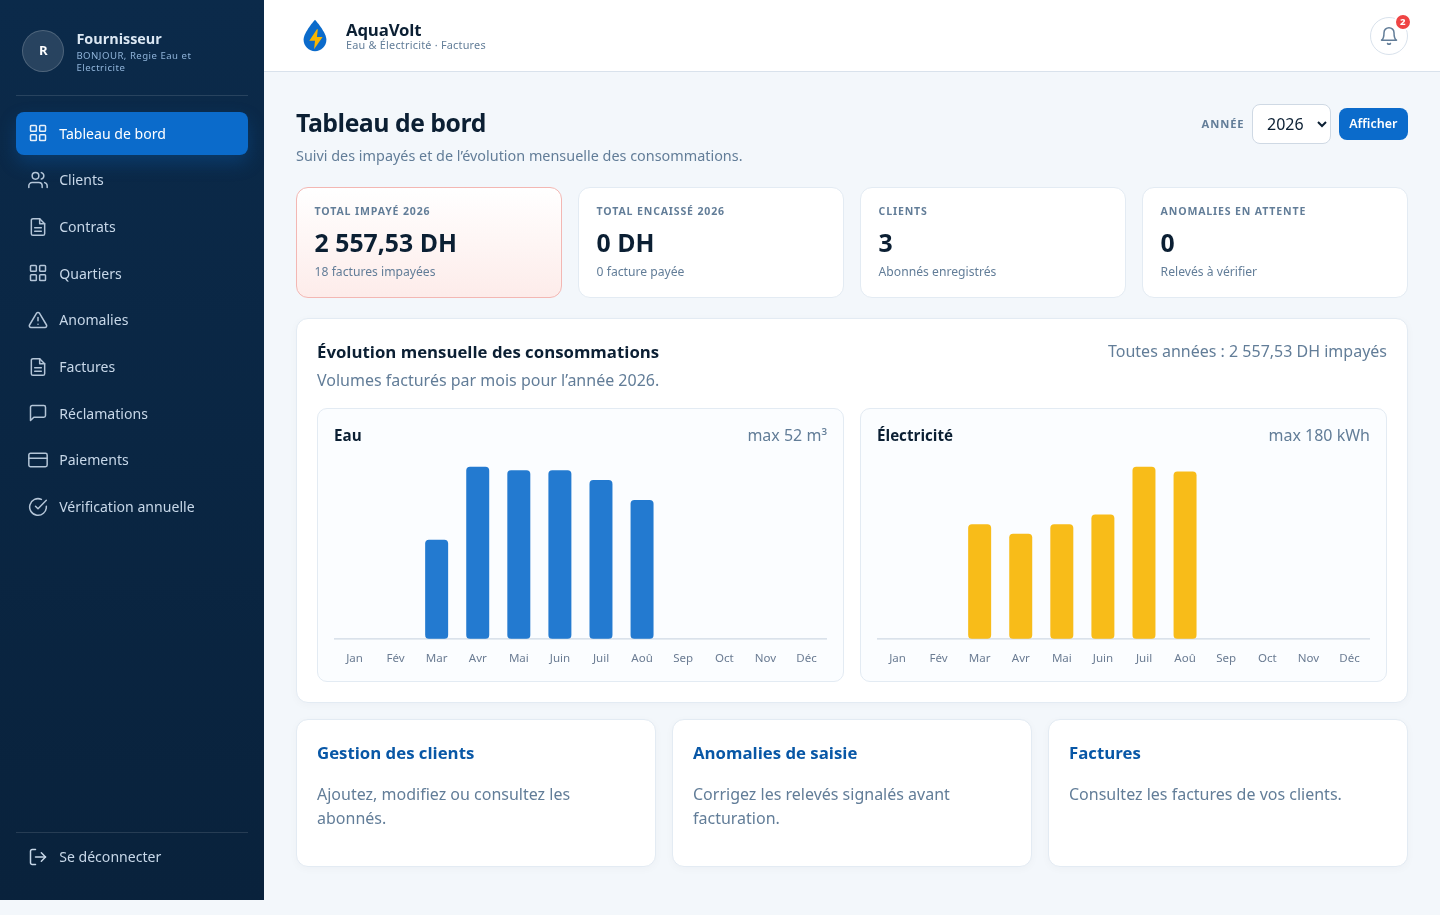
\includegraphics[width=0.95\textwidth]{../tests/final/desktop/06_supplier_dashboard.png}
  \caption{Tableau de bord du fournisseur}
  \label{fig:dashboard}
\end{figure}
